%=========================================================================
% (c) Ivan Ševčík, 2015
abb:
EEG,
PC,
CPU,
GPU,
API,
SDK,
DWT,
DFT,
FFT,
2D,
3D,
DSP - digital signal processing

%TODO: articles and commas check, check, check..
%TODO: http://www.grammarbook.com/punctuation/commas.asp
%TODO: conjuctive adverb
\chapter{Introduction}
%TODO: citations in this chapter too
% Uvod do temy
The brain is central organ of human nervous system and as such has very
important role in almost every activity. However, its complexity makes it
difficult to study and understand. Rapid development of computers in recent
decades provided partial solution to this as it allowed for mapping and
monitoring both structure and activity of brain with high precision.

% Aktualny stav, problemy
But raising interest in EEG technology and brain-computer interfaces also means
that there is an evident need for user interfaces and applications capable of
processing these signals for various purposes. One such purpose is visualization
that allows researchers and users to better comprehend measured data as these
are usually just binary values that may be represented as integer or decimal
numbers, therefore hard for humans to interpret. Another issue is that,
generally, users are not interested in raw values but in some features that
signal carries such as intensity at certain frequency or specific patterns that
represent certain activity performed by measured subject.

% Ciele
The goal of this work is to create an application implementing several
methods for signal processing and visualization, including classification by
frequency, charts showing wavelet of measured signal in time domain, and both
two and three-dimensional models displaying brain acitivity. Another important
task will be to create intuitive and clean, yet highly customizable graphical
user interface, which will be responsive also for real-time signal inputs. The
application should, however, be able to process also large offline data measured
earlier without noticeable performance decrease.

% O com to tu je
The text is structured into chapters that start as a general theory and
progressively get more specific, concluded by an application concept and
implementation. In chapter \ref{humanBrain}, background information about brain
and methods for measuring its activity, specifically EEG, is presented. Moving
on, chapter \ref{appProcVis} provides required foundations of signal processing
and computer visualization. Chapter \ref{eegProcAndSol} puts these general
methods into context of EEG analysis and also contains reviews of few existing
solutions in field that serve as an inspiration for this work. The concept is
introduced in chapter \ref{concept} and eventually transforms into
implementation, which is described in chapter \ref{implementation}.
 
\chapter{Human brain} \label{humanBrain}
Brain is a central unit of human nervous system and has important role in almost
every aspect of life. It performs both conscious tasks and automatic operation
of vital organs, like breathing, maintaining blood pressure and releasing
hormones. It also processes all sensory inputs, such as odors, sounds or light,
interprets them and make associations with representations preserved in memory.
\section{Brain biology}
The biology of brain is complex and many processes that are ongoing within it
are still not well understood. In this section we will, therefore, provide only
very brief introduction to its anatomy and communication mechanisms that are
relevant for this work.
\subsection{Anatomy}
From anatomy point of view, we are interested in cerebrum, which is the
outermost structure of brain. It is divided into two separate hemispheres
bridged by bundle of fibers. The cerebrum is associated with higher-order
functioning and the control of voluntary behavior. This include thinking,
perceiving, planning and understanding language. The cerebrum is covered with a
sheet of tissue called cerebral cortex, which is further divided into regions
that are functionally differentiated and called lobes. There are four lobes,
each with different role. The frontal lobe is where initiation and coordination
of motor movements take place, along with higher cognitive skills, such as
thinking, planning and organizing. It is also important for personality and
emotional makeup. The parietal lobe is responsible for processing sensory
inputs, attention, language and spatial orientation. The occipital lobe helps
process visual information and assists with recognition of shapes and colors.
Finally, the temporal lobe is region where auditory information is processed and
the information from other senses is integrated. It also has a role in
short-term memory and in learned emotional responses. \cite{brainFacts} The
Figure \ref{fig:brainAnatomy} shows all discussed structures on the model of brain.

%TODO: footnote is on other page
\begin{figure}[ht]
	\centering
	\includegraphics[width=1\linewidth]{fig/BrainAnatomy.jpg}
	\caption[Caption for LOF]{Brain anatomy\protect\footnotemark}
	\label{fig:brainAnatomy}
\end{figure}
\footnotetext{Image source \texttt{http://www.compelvisuals.com/wp-content/uploads/2013/12/BrainAnatomy-Newsletter.jpg}}

\subsection{Neurons}
The nervous tissue is made of cells called neurons that communicate with each
other and represent basic working units of brain. The neuron consists of cell
body, dendrites and an axon. The cell body contains nucleus and cytoplasm, and
produces peptides required for communication. Dendrites extend from cell and
receive signals from other neurons through synapses -- contact points where
axons of other neurons connects to dendrite. The axon is used to transmit
electrical impulses outward from neuron. These electrical impulses originate
from sudden change of electrical potential caused by flow of ions through cell
membrane. The change, called an action potential, then passes along axon's
membrane and upon hitting its end releases neurotransmitters in nerve terminals.
The neurotransmiters diffuse across synapse and bind to receptors on the surface
of target cell's dendrite, which causes response in target.\cite{brainFacts}

\section{Electroencephalography}
The nature of human nervous system, as has been presented, is electrical. It has
been observed that the variation of surface electrical potential measured on the
scalp is related to amount of activity in underlying brain structures. EEG is a
method for measuring these potential variation using an array of electrodes
placed on measured subject's scalp and recording them for later processing.
\cite{eegClass}

The main advantage of EEG over other methods is speed as it can record respond
to stimulus within fractions of a second. \cite{eegFund} Applications of EEG
include:
\begin{itemize}
  \item Research -- monitoring during cognitive and motoric tasks
  \item Medical -- diagnosis of brain diseases
  \item Human computer interaction -- performing commands using brain activity  
\end{itemize}
Recently, the EEG based devices also penetrated consumer market and users can
monitor brain activity at home, play simple games and control toys using
their thoughts. 
%TODO: (footnote-quadcopter)

\subsection{Basic principles}
It is impossible to measure or distinguish electrical activity of each neuron
with EEG, because these are asynchronous and cancel each other out. 
What EEG measures is summated potential of neuronal activity, which includes
spontaneus electrical activity of the cerebral network and cortical responses to
external and internal events. The responses to events, characterized by their
onset latency and voltage amplitude, are reffered to as \emph{event-related
potentials} and are either result of physical stimuli, or behavioral responses.
\cite{bcComm}


\subsection{Measurement equipment}
The setup used for encephalographic measurements usually consist of: 
\begin{itemize}
  \item Electrodes with conductive media
  \item Amplifiers with filters
  \item A/D converter
  \item Recording device
\end{itemize}
% Electrodes
The electrodes exists in various forms but in this work we will focus on
headsets and electrode caps, such as one displayed in Figure \ref{fig:eegCap}.
These caps usually consists of small discs serving as electrodes made
of very conductive material, such as gold, silver or stainless steel. Commonly
used electrodes are made of Ag-AgCl disks with diameter of \SIrange[range-units
= single]{1}{3}{\mm} and have long leads that can be plugged into an
amplifier. \cite{eegFund} The discs are in direct contact with scalp and can already
measure electric potential produced by brain. However, conductive media in form of a
gel or paste is often used to increase conductivity even more by lowering
contact impedance and improve readings at the lowest level. It also helps
electrodes to stick to surface so accidental shift from position is less likely.

%TODO: footnote is on other page
\begin{figure}[ht]
	\centering
	\includegraphics[width=1\linewidth]{fig/eegCap.jpg}
	\caption[Caption for LOF]{Electrode cap\protect\footnotemark}
	\label{fig:eegCap}
\end{figure}
\footnotetext{Image source \texttt{http://www.psychologie.uzh.ch/fachrichtungen/plasti/Labor/EEG-03.jpg}}

% Cap
The electrodes are pre-mounted on a silicon cap in locations according to
standardized placement system, which will be discussed later in this section.
This both speeds up the setup stage and allows for unified mapping of electrodes
to head surface, but fails to account for different shape and features of each
individual's head. \cite{eegFund} This problem is usually solved by involving a
method for finding 3D coordinates of electrodes on the head. Such methods
include using magnetic field digitizer or elaborate algorithms that can
calculate position of each electrode from few distance and angle measurements by
utilizing specific properties of standard placement system. \cite{rapidPos}

% Amplifiers
The strength of signal measured by electrodes is in order of microvolts and
normally range from \SIrange{10}{500}{\uV}. \cite{neuralAmp} An amplifier is,
therefore, needed to bring the amplitude to higher levels so it can be processed
by other electrical circuits and components. The requirements on amplifiers for
use with EEG are high as they have to provide amplification only for physiological
signal, which should not be distorted in any way, reject superimposed noise and
interference signals, and protect both the equipment and measured subject from
current surges. Amplifiers conforming to these requirements are known as
\emph{biopotential amplifiers}. \cite{biopotAmp}
% Filters
A bandpass filter is then used to limit frequencies into a certain range of
interest. In some cases it may be already a part of an amplifier.
Another common filter is notch filter which is used to filter out noise
at frequency of power line. Depending on country, it may be set to
\SIlist[list-units = single, list-pair-separator = { or }]{50;60}{\Hz}.
\cite{deltaCompNREM} Such filter is only used if it is desirable to keep also
high frequencies as the interesting frequency bands usually lies bellow this
threshold.
% Trend in amplifier miniaturization
The trend in development of neural recording devices is heading in direction of
fully implanted systems(konzultovat). Consequently, energy efficient amplifiers
are being designed lately that are very small in size, may run on battery for
long periods of time and dissipate only little heat so they don't damage
surrounding tissue. \cite{neuralAmp}

% A/D converter
An A/D converter unit is then used to convert analog values to digital
representation. The converter should have resolution of at least 12 bits and
ideally 16 bits or more. With high number of electrodes, analog multiplexers are
sometimes used to lower the number of necessary converter units at the expense
of limited update frequency. The sampling frequency should be at least double of
the highest recorded frequency, for example the upper frequency limit set for
bandpass filter. This is known as Nyquist-Shannon sampling theorem and is
fundamental for correct signal reconstruction without aliasing artifact. The
preferred sampling frequency is \SIrange{256}{400}{\Hz}. \cite{guidDigEEG}

% Recording device
Converted samples from A/D converters are then stored in memory for further
processing which will be discussed in another part of this section
\ref{sub:dataAnalysis}. A recording device may be represented by a computer or a
different piece of specialized equipment. The computer can be additionally
equipped with digital signal processor unit so that CPU load is lower and can be
used for other tasks.

\subsection{Electrode placement systems}
\label{ssec:elPlacement}
% Uvod
The need for standardized electrode placement was evident as early as 1947 when
the first International EEG congress held place in London. Various methods of
standardization were proposed and this effort finally resulted in the definition
of 10-20 electrode system in 1958 by H.H. Jasper. \cite{placeSys} 
% Popis 10-20
This system consists of 21 electrodes placed evenly between certain landmarks
and the labels of electrodes are derived from cerebrum lobes above which they
are located. The first contour can be found by connecting inion and nassion.
Inion is small pretuberance at the back of the head and nassion is located just
above bridge of the nose. The length of this line is measured and electrodes are
placed along it using following procedure. First electrode -- Fpz, is placed at
10\% of length from nassion. The electrodes Fz, Cz and Pz are placed in this
order from front to back with spacing of 20\% of length. Fz and Fpz are also
spaced by 20\%. Last electrode -- Oz, is placed at 10\% of length from inion
which equals 90\% of length from nassion. It should be clear now why the system
is called 10-20. The rest of electrodes are placed in similar fashion and this
can be seen at image.. %obrazok do prilohy

% Popis 10-10
The 10-20 system offers only limited resolution but it was sufficient at the
time of its creation because the main limiting factor was technology. However,
with technological advances in computers and signal processing, using more than
21 channels became feasible and, naturally, many sought to take advantage of
higher resolution. With more electrodes than what is 10-20 model capable of
accommodating, first extension to standard placement system was needed. The
extension, named 10-10 system, was proposed in 1985 and extended the number of
electrodes to 74. It uses additional coronal contours lying halfway between
original contours and combines the labels of these original contours to create
new label. For example, the contour lying between original contours F and C will
be labelled FC. \cite{placeSys} The position of electrodes according to this
system are shown..
% obrazok do prilohy

% Popis 10-5
The 10-5 electrode placement systems further extends the 10-10 system to allow
even higher number of channels to be used as systems with over 128 channels are
not uncommon any more and have become commercially available. The idea in
placement of new electrodes is similar to how 10-10 system extends from 10-20,
creating coronal contours halfway between the original ones. The nomenclature
uses naming in similar fashion as geographical directions. For example,
direction between North and North-West is labelled as North-North-West and so
contour between C-contour and CP-contour will be labelled CCP-contour.
This doubles the number of contours and also the number of electrodes in contour
is doubled, increasing the number of electrodes by approximately 4 times.
The total number of possible locations is around 345 and may vary depending on
how many electrodes are included for the most inferior rows. \cite{placeSys}
This system is in proposition stage and is yet to be recognized as standard, but
it is currently only work in this area, therefore can be considered as relevant
and some equipment already adheres to it.

\subsection{Measurement procedure}
Before measurement the electrodes are cleaned thoroughly to remove any
impurities that could have an impact on it. The skin is also cleaned from oils
and brushed from dried parts. It is important to adhere to strict hygiene as
this might cause irritation and inflammation, and with repeated measurements may
develop into an infection.\cite{eegFund} The subject is then seated comfortably
to eliminate any unnecessary movement, because it could spoil the measured data.
(cite?) Electrodes or cap are placed on subject's scalp and recording can begin.
In case of a research oriented session, the subject is usually instructed to
perform specific tasks such as imagining moving certain part of body, rotating
an object in 3D or focusing on specific part of display. \cite{bcComm} For other
purposes, such as medical diagnosis, subjects may be monitored while laying on
their back with closed eyes or during sleep.

\subsection{Data analysis} \label{sub:dataAnalysis}
The recorded data are subject to further processing using numerical filters and
transforms to improve signal-to-noise ratio and extract desired features. 
% Clasification by frequency band
One such feature is brain activity at certain frequency. The frequency of brain
waves range from \SIrange{1}{150}{\Hz}. This range can be further divided
into six common categories\cite{dominantF}:
\begin{itemize}
  \item Delta waves -- below 4 Hz
  \item Theta waves -- between 4 and 8 Hz
  \item Alpha / Mu waves -- between 8 and 13 Hz
  \item Beta waves -- between 13 and 30 Hz
  \item Gamma waves -- between 30 and 80 Hz
  \item High gamma waves -- above 80 Hz
\end{itemize}
A healthy person exhibits brain waves mostly in the first four categories. Each
band is related to certain group of activity in brain and can be used for
diagnosis as abnormal resting powers in certain bands were linked to various
mental and physiological diseases. \cite{dominantF} Delta waves are normally
distributed over scalp and may be significant during deep sleep, in childhood or
in serious organic brain disease. \cite{eegClass} Theta waves are related to
cognitive tasks such as working memory and error monitoring tests. Alpha power
is increased during inattention and lack of visual input, therefore related to
perception. Mu power, on the other hand, is linked to movement and is decreased
when person performs a motor action. The distinction between alpha and mu waves
is made by considering the location of electrode. While alpha waves form at the
back of the scalp, mu waves can be observed in a strip of brain from ear to ear
called motor cortex. Finally beta waves are low amplitude, high frequency waves
that have power reduced at the onset of movement, rebound if the movement is
sustained and are enhanced if the movement is suppressed. \cite{dominantF}

% Classifier reference
Many researchers proposed implementation of classifiers capable of identifying
these frequencies in signal using various approaches. One such method that is
used in this work is described in detail in section \ref{eegClassifier}.

% Classification by pattern
Another set of features are patterns that represent certain activity more
clearly than classification by frequency. For example, the imagined movement of
finger can be distinguished from imagined movement of leg with this method. The
classification accuracy is, however, highly individual and the classification
system usually needs tuning or calibration process for each user. \cite{bcComm}
Common approach to this problem is training a neural network that can classify
patterns in brain waves with accuracy high enough for normal usage.

\chapter{Approaches to signal processing and visualization} \label{appProcVis}
%TODO: some introduction to the chapter

The term signal processing will be from now on restricted to digital signal processing as the processing will be performed in software. Likewise, the term signal will be restricted to a discrete-time signals represented as sequence of numbers. 

(DSP3 = Digital Signal Processing, Third Edition, John Proakis, Dimitris Manolakis)
\section{Signal processing} \label{sec:sigProc}
As presented in section \ref{sub:dataAnalysis}, signal processing is important
step to ease analysis of recorded data by filtering out noise and selecting
signal features. This section will, therefore, provide general information about
methods of signal processing and section \ref{sec:implFIRfilters} will provide implementation details. 
 
%\subsection{Nyquist-Shannon theorem} maybe

\subsection{Discrete Fourier transform}
Discrete Fourier transform is an operation that produces corresponding frequency spectrum for any given sequence of numbers. Formally the DFT is defined by Equation \ref{eq:DFT} where the sequence $x(n)$ represents the input, usually a signal (401, DSP3). 

\begin{equation}
\label{eq:DFT}
	X(k) = \sum\limits_{n=0}^{N - 1}x(n)e^{-2 j \pi k n /N} \qquad 0 \leq k \leq N-1
\end{equation}

The product of the DFT is a new sequence $X(k)$ of complex numbers equally spaced in frequency domain. Each number represents a sample in the frequency spectrum. Because the numbers are equally spaced, each sample belongs to a certain frequency interval that is often refereed to as a frequency bin. A bin resolution, that is the length of each frequency interval, can be determined through Equation \ref{eq:DFTres} where $f_s$ is the sampling frequency of the input signal. 

\begin{equation}
\label{eq:DFTres}
bin_{res} = \frac{f_s}{N}
\end{equation}

The direct computation of DFT is inefficient and contains repeating, and thus redundant, operations. Because of that, a more efficient algorithm called fast Fourier transform is used in practical applications. The FFT algorithm takes advantage of symmetry and periodicity to reduce number of operations needed to compute the result. The number of complex multiplications can be used as a criterion when comparing the efficiency of the DFT and FFT. Indeed, while the DFT requires $N^2$ multiplications, the FFT algorithm requires only $(N/2)\,log_2N$ multiplications to produce the exactly same results. For example, the speed is improved $204.8$ times for a 1024 point DFT. (459, DSP3)

\subsection{Filters in general}
A filter in the broadest context is any system that modifies certain frequencies relative to others. For the purposes of this thesis the term filter can be narrowed to a system that passes certain frequency components and totally rejects others (439, DSP). All discussed filters will be casual. A system is casual, if for every choice of $n_0$, the output sequence value at the index $n = n_0$ depends only on the input sequence values for $n \leq n_0$ (21, DSP). The stability of filters will be also discussed in section \ref{ssec:FIRandIIR}. A system is stable if and only if every bounded input sequence produces a bounded output sequence. The input $x[n]$ is bounded if there exists a fixed positive finite value $B_x$, such that(21, DSP)
\begin{equation}
	|x[n]| \leq B_x < \infty\text{,\qquad for all n.}
\end{equation}
The system is stable if for each bounded input there exists a fixed positive finite value $B_y$, such that(22, DSP)
\begin{equation}
	|y[n]| \leq B_y < \infty\text{,\qquad for all n.}
\end{equation}

The filtering can performed as convolution of the input signal with filter's impulse response in time-domain. Another, equivalent method is to first perform DFT for the input signal, multiply the obtained spectrum with filter's frequency response and perform an inverse DFT. 

\subsection{FIR and IIR filters}
\label{ssec:FIRandIIR}
One of the most important decisions when considering the use of filters is the decision between finite and infinite impulse-response filters. These are two fundamentally different groups of filters with many differences, which will be briefly discussed. The major difference between the systems can be seen from difference equations \ref{eq:FIRsystem} and \ref{eq:IIRsystem} (500, DSP3). While the FIR system uses only current and past input values, the input to the IIR system includes also previous output values.

\begin{align}
	\text{FIR system\qquad} &y(n)= \sum\limits_{k=0}^{M-1}b_kx\,(n-k) \label{eq:FIRsystem}\\
	\text{IIR system\qquad} &y(n)= -\sum\limits_{k=1}^{N}a_ky\,(n-k) + \sum\limits_{k=0}^{M}b_kx\,(n-k) \label{eq:IIRsystem}
\end{align}

Another difference between the two groups involves stability. The FIR systems are inherently stable from the definition but great care must be taken to design a stable IIR system. The IIR systems also suffer from limited precision of numbers in computer memory. An error accumulates over time due to the feedback. 

Considering the properties of both filter types and difficulty of implementation it was chosen to further use only FIR filters.

\subsection{Low pass and high pass FIR filters}
A low pass filter is a system that ideally passes only frequencies below a specified threshold called cutoff frequency $f_c$. Accordingly, a high pass filter is a system that passes only frequencies higher than the threshold and attenuates the others (331 DSP3). 

The filter is created by finding the coefficients $b_k$ for equation \ref{eq:FIRsystem}. This can be done in general by designing the desired frequency response in frequency domain and using inverse Fourier transform to obtain filter's impulse response $h(n)$ which represents the coefficients. However, the low pass and high pass filters are so common that the impulse response can be obtained using equations \ref{eq:lowPass} and \ref{eq:highPass} where $\omega_c = 2 \pi f_c$ and $M$ is the filter's length(472, DSP).

\begin{align}
\text{Low pass\qquad} & h(n) = \begin{cases}
\frac{\sin \left( w_c \left( n - M / 2 \right) \right)}{\pi \left( n - M / 2 \right)} & \qquad n \neq M / 2 \\[0.2em]
2 f_c & \qquad n = M / 2
\end{cases} \label{eq:lowPass}\\[1em]
\text{High pass\qquad} & h(n) = \begin{cases}
-\frac{\sin \left( w_c \left( n - M / 2 \right) \right)}{\pi \left( n - M / 2 \right)} & \qquad n \neq M / 2 \\[0.2em]
1 - 2 f_c & \qquad n = M / 2
\end{cases}\label{eq:highPass}
\end{align}

\subsection{Window functions}
In general, the filter's impulse response obtained through inverse Fourier transform is infinite in length. It must be, therefore, truncated at some point, say at $n = M-1$, to yield an FIR filter of length $M$ (624, DSP3). The truncation is equivalent to multiplying the infinite impulse response by a rectangular window  which is defined by Equation \ref{eq:rectWind}.

\begin{equation}
\label{eq:rectWind}
w(n) = \begin{cases}
1 &\qquad 0 \leq n \leq M-1\\
0 &\qquad \text{otherwise}
\end{cases}
\end{equation}

However, such truncation produces undesired effects in frequency response. For example, let's consider an FIR low pass filter with cutoff frequency $f_c=\SI{0.4}{\Hz}$ and length $M=31$. The left graph in Figure \ref{fig:filterRiples} depicts the frequency response of such filter after truncation. It can be seen that the gain at frequencies below cutoff fairly fluctuates and also the attenuation at frequencies above cutoff is relatively weak. The graph on the right side shows the frequency response for the exact same filter but the truncation was done using Hamming window. Clearly, the fluctuations are much smaller, almost invisible at this level of detail. Also the filter better attenuates undesired frequencies. However, this comes at a cost of a longer transition to reach the stop band. While the filter with rectangular window reaches stop band at frequency a little over \SI{0.4}{\Hz}, the filter using Hamming window gets to stop band at approximately \SI{0.5}{\Hz}. Therefore, a choice must be made but the advantages of using window function usually outweigh the disadvantages.

\begin{figure}[ht]
	\centering
	\includegraphics[width=1\linewidth]{fig/filterRiples.pdf}
	\caption{Comparison between filters with Rectangular and Hamming window}
	\label{fig:filterRiples}
\end{figure}

The window function in essence weighs samples entering the filter so that transition into truncated area is smooth rather than sudden as in the case of rectangular window. The Equation \ref{eq:hammWind} defines the already discussed Hamming window and Equation \ref{eq:blackWind} defines another commonly used Blackman window (626, DSP3). The definitions are only for $0 \leq n \leq M-1$ as the rest of the impulse response is still truncated.

\begin{align}
\text{Hamming window\qquad}& w(n) = 0.54 - 0.46\cos \frac{2 \pi n}{M -1} \label{eq:hammWind}\\
\text{Blackman window\qquad}& w(n) = 0.42 - 0.5\cos \frac{2 \pi n}{M - 1} + 0.08\cos \frac{4 \pi n}{M - 1} \label{eq:blackWind}
\end{align}

\section{Data visualization methods}
So far, only methods of measuring and processing data from EEG have been
discussed but the primary goal is to visualize them. Therefore, this section
will discuss methods of data visualization using computers and common
display devices such as monitors and screens, and how these visualizations can
be used to help humans analyze data more easily.

\subsection{2D representations}
Display devices and other media used for presenting information have mostly
two-dimensional nature. This has great implications for how the data are usually
visualized and manipulated. The most natural representations are those that are
already organized spatially as two-dimensional, without needing any projections
and mappings. It is still possible to add the next dimensions through usage of
colors, different shapes and sizes, but the diagram was from start intended to
take on two-dimensional form. The most commonly used diagrams are based on
graphs and charts, although schematics and maps are also popular.

The graph is type of a diagram made of interconnected objects. The connection
may be represented by a line or curve which may be directed, meaning that it
goes only one way. Graphs are usually used for visual representations of data
where individual entities and their relations can be recognized, for example a
network of roads between cities, but they are also usefull for displaying
hierarchies.

The chart is a visual representation of data useful for plotting, categorizing
and showing trends. It may come in many forms, like bars or lines drawn in an
area designated by axes with scales, or slices of a pie. Choosing the most
suitable one, so that the most significant fact stands out, is important step in
data visualization.

\subsection{3D models}
The world and objects within it are perceived by humans as three-dimensional
and, therefore, it is preferable to use three-dimensional representations of
objects called 3D models. However, there is lack of technology for displaying
such representations truly three-dimensionally, with holograms being the most
advanced one. Because of that, the models must be projected into two dimensions
so that they can be displayed using existing devices. This is done using
projection matrices during process called rendering. The two most common
projections are orthogonal and perspective.

There are multiple ways to create the 3D model. It is possible to scan real
world objects by various means, such as tomography and optical surface imaging.
Another method is to use special modeling software and reconstruct the model from basic
primitives. The model may have defined volume using volumetric or voxel
representations, or it can be just a surface of an object which is usually
represented by a mesh. A mesh is a collection of points in 3D space called vertices
which are connected to form basic primitives, like triangles and polygons.

\section{Programmable graphics pipeline}
\label{sec:pipeline}
A graphics pipeline represents the process of rendering and its stages. The
input data in form of vertices, colors and other information represent the input to the
first stage which processes and passes them down the pipeline to another stage.
The result of final stage is rendered image of scene. Before programmable
pipeline was developed, programmers could only use vendor defined operations and
combine them to create their application which imposed certain constraints on
what could be done. This was called a fixed pipeline, because the action
performed by each stage was fixed and could be only modified through parameters
or states. With introduction of programmable pipeline, it was possible for
programmers to step into rendering process in several places and define their
own techniques. The custom programs that have become part of pipeline are called
shaders. In following text we will present the three most important types of
shaders with respect to their position in pipeline. The Figure \ref{fig:OpenGLPipeline} displays OpenGL graphics pipeline. The terminology used in this section is also
according to OpenGL but the basic principles are similar for most of the graphics card APIs. 

\begin{figure}[ht]
	\centering
	\includegraphics[width=1\linewidth]{fig/OpenGLpipeline.pdf}
	\caption{OpenGL 3.3 programmable graphics pipeline}
	\label{fig:OpenGLPipeline}
\end{figure}

\subsection{Vertex shader}
A vertex shader is at the very front of graphics pipeline, just after primitive
processing. It allows to modify properties of vertices before they enter
geometry shader or primitive assembly stage. The input to vertex shader is
single vertex with all related information. Typical usage of this stage consists
of applying projection and transformation matrices, Goraud shading,
displacements and controlling particle effects.

\subsection{Geometry shader}
A geometry shader, if present, is executed right after vertex shader but instead
of working with isolated vertices, it works with whole primitives like points,
lines and triangles. It may perform transformation from one type of primitive to
another and also emit completely new geometry. For example, it is possible to
have as input only one point and output may be circle with that point as a
center made of varying number of triangles, depending on how far from camera
the point was. This not only saves time-expensive transport operation between
CPU and GPU, but also optimizes performance by dynamically lowering details.

\subsection{Fragment shader}
A fragment shader works with individual pixels, produced by rasterizer after the
primitives have been assembled. However, the three-dimensional information have
not been discarded yet and is accessible during processing. This allows to apply
three-dimensional effects on the finest level, such as phong shading. The output
of this program is single color that will be displayed on that specific pixel.

%TODO eegProcAndSol chapter changed, change also introduction
%\chapter{EEG specific procedures and solutions} \label{eegProcAndSol}
\chapter{Overview of existing solutions}
\label{existSol}
This section will analyze existing solutions by focusing on their user interface, features, extensibility and intuitiveness.

\subsection{Emotiv}
Emotiv is a company specializing in area of EEG devices for consumer market.
Currently they offer two options -- 14 channel EPOC and 5 channel Insight
headsets. These headsets come with built-in amplifiers, filters and A/D
converters, and communicate wirelessly with computer through bluetooth. As
we lack necessary hardware, we will review this solution from videos posted on
the internet by users who own the headset and from information available on
company's website.

The headset is accompanied with software, which has to be bought through store
separately. On one side, the store allows the developers to create new
applications independently but as a result, there is lack of single, unified
user experience. This is caused not only by different styles the authors of each
application used, but also because each application have its own set of
settings, controls and displays, many of which are duplicated between
applications. For example, a chart with signals from electrodes is included in
both TestBench and 3D brain activity map applications. There is also another
brain activity map that displays each frequency band in 2D and the settings,
such as gain factor and buffer size are not shared in any way between
applications, resulting in different behavior, which can be quite confusing.
However, the focus on ordinary computer users can be felt as the applications,
when considered as standalone products, are visually nice, polished and
user-friendly.

Feature-wise, the applications are ranging from visualization software and data
importers to games. One important feature that seems to be missing from most of
the applications is lack of any control of time, meaning they are only able to
display current values. This is very limiting factor for data analysis, as one of
basic tasks performed is comparing data. Being able to do so between two or more
moments in time is definitely desirable. The SDK for creating new applications
is freely available, so anyone can start developing.

\subsection{Svarog}
Svarog stands for Signal Viewer, Analyzer and Recorded on GPL and is
implemented in Java. It is intended for use as an advanced analysis tool capable
of both online and offline signal viewing and processing. The data may be in any
data format as long as SignalML description is provided.

The application offers only basic visualization methods. Main GUI element
visible after starting the program is chart with EEG wavelets. It allows to
modify amount of space between signals, the amplitude and time scale, select
part of a signal on one or multiple electrodes, zoom in or out and an
interesting tool is FFT viewer that can show FFT for segment of signal in
superimposed window. Another interesting element is time-frequency map that is
used for showing results of matching pursuit algorithm that is one of available
processing tools. Time is on horizontal axis, frequency on vertical axis and
amplitude is represented by color in range from blue to red. However, there is
no brain map and other visually more appealing elements.

The GUI is sometimes cluttered with too many options, which could have been
hidden in some advanced view, but overall is clean, quite customizable and
informs user about progress of operations. It also allows to create auxiliary
signal plots, which are useful for signal comparison. With too many signals
the responsiveness degrades, probably because the plots are rendered in software.

%TODO: aky cas pouzivat.. minuly, pritomny, buduci.. was, is, will, should,.. asi pritomny bude najlepsie - navrh je hotovy a prezentujem ho
\chapter{Concept and design} \label{concept}
It is usually a good idea to create a concept before implementing a non-trivial project. A concept development process helps to make clear which are the important parts of the project and how they are going to communicate and work together to provide desired results. The concept also helps to maintain a good code structure and class hierarchy. Therefore, the text in this chapter defines the concept that will be used during development of the application.

\section{Logical division}
The first step in concept creation is to analyze the problem and divide it into smaller ones. It is possible to split the whole application into individual subsystems such as:
\begin{itemize}
	\item GUI
	\item Model importer
	\item 3D math library 
	\item Signal input module
	\item Signal processing module
	\item Rendering system
	\item Animation system
\end{itemize}

The following sections will address each subsystem individually.
\subsection{User interface}
A user interface is an important part of any application as it allows users to interact with it. The user interface provides both an input to the and an output or feedback from the application.

The user interface may be created using different techniques. One way to provide user interface is by using graphical elements, hence the name graphical user interface. The terminology and appearance of elements varies between platforms but there are usually container-like objects called windows that provide a display area also known as canvas for other elements such as buttons, scrollbars, text labels, editable fields, etc. The elements can be grouped and create layouts that are visually appealing. Another very common element that can be usually found near top of the window is menu bar. It provides fast access to most of the functionality and its unfolding structure saves space for other elements. 

An important question to ask is who will be the targeted audience. The difference between targeting ordinary users and researchers can be seen in section \ref{existSol}. The original assignment predetermines this work to be used primarily for academic purposes. Nevertheless, the ideas of visually appealing graphical elements and friendly user interface will be also incorporated as they can dramatically improve the experience.

A common approach to GUI design is to first create a simple model called mockup. The mockup can be drawn on paper or created using specialized software. It should capture all the important elements and define their position and purpose. The GUI is then created to resemble to mockup using a technique that is specific to the platform, such as Qt. The resulting GUI is presented in section \ref{sec:GUI}. 

\subsection{Model importer}
Loading 3D mesh models into memory in a representation that may be used for rendering is a non-trivial task. This is further complicated by a diversity of file formats that are used to store 3D models. One of the most popular file formats is \texttt{Wavefront .obj} file. It can store whole scenes with multiple objects that are represented using polygons. Most of the 3D modeling software also allows to export the model using solely the triangles that can be rendered directly by OpenGL. Another advantage of \texttt{Wavefront .obj} file format is that it uses ASCII and human readable data representation. The Listing \ref{lst:ObjFile} shows an example of \texttt{.obj} file that defines a triangle. Due to the stated properties, the format was chosen to store the model of brain.

\lstset{captionpos=b, caption=The .obj file example, label=lst:ObjFile}
\begin{lstlisting}
	# object Triangle
	v  -0.5 0 0
	v  0.5 0 0
	v  0.25 0.5 0
	# 3 vertices
	
	g Triangle
	f 1 2 3 
	# 1 face
\end{lstlisting}

The model importer has to be able to open \texttt{.obj} file, list the stored objects, and provide data for each of them. The data, such as vertex positions, are then passed to Rendering system that will render the object. A Tiny obj loader library is a perfect solution for our needs. It is light-weight C++ library implemented by single file that is simply compiled with the rest of the application and has no dependencies except for C++ STL. After loading the triangulated model from \texttt{.obj} file, the geometry and other information is conveniently stored inside STL \texttt{vector} that can be used directly by rendering system.

\subsection{3D math library}
A 3D math library is required in order to manipulate objects and 3D space. At least support for translation, rotation and projection is needed. The library should also include algorithms for creating transformation matrices used by OpenGL. Naturally, the data structures such as vectors, matrices, and basic geometry should be part of the library.

The OpenGL Mathematics library covers most of these requirements. It provides the same functionality and data types that are found in GLSL language plus additional useful features such as the matrix transformations, quaternions, data packing, etc. The only drawback is that the library does not provide any 2D or 3D objects.

\subsection{Signal input module}
The EEG data is required by the application in order to produce actual results. The problem is that there are many file formats actively used, some of which are specific to single medical laboratory or recording equipment. However, there is an effort to create single standard file format. The European Data Format (EDF) is an example of such effort. The format stores the electrode signals in form of data records which are time-continuous blocks of samples. The format also provides additional information, such as a duration of data recording and the whole file, maximum and minimum for the signal amplitude, information about a patient, etc. 

The EDF format was chosen to be primary source of EEG data because of its popularity and versatility. However, the data format is not trivial to read. Because of this, an already existing C library was used. The EDFlib supports not only the original EDF format but also its extension EDF+ and derivations BDF and BDF+. The library also has some limitations, such as that the whole file must be continuous but this support is not required by our application anyway. After opening a file in the EDF format, each signal can be read individually as a stream. The signal input module then provides the data to the rest of the application in an internal format.

\subsection{Signal processing module}
The signal processing module implements filters and transformations presented in the section \ref{sec:sigProc}. The discrete Fourier transform is usually implemented as a fast fourier transform (FFT). There are already many libraries implementing FFT. One such library is Kiss FFT and it was chosen due to its simplicity, compact size, and benevolent license. However, no simple library could be found that implements FIR filters. It was decided that rather than including large DSP library with lots of dependencies, the few filters that are necessary will be implemented anew. The section \ref{sec:implFIRfilters} provides implementation details.

\subsection{Rendering system}
The rendering system provides the necessary functionality to produce a visual output. It is the most complex part of application and can be further divided into:
\begin{itemize}
	\item General rendering support for OpenGL primitives
	\item 3D mesh object rendering support
	\item Electrode visualization
	\item EEG data visualization
\end{itemize}

The whole rendering system is hardware accelerated in order to provide a good performance. The hardware acceleration is provided by the OpenGL API and graphics pipeline introduced in section \ref{sec:pipeline}. Because of that, a shader program is needed for each rendering task. The implementations details of shader programs are discussed in section \ref{sec:implRendering}. A Unishader library is used to load and use the shader programs. The Unishader is previous work by authors of this thesis that creates an automatized wrapper around OpenGL focusing on the shader support. It greatly simplifies the setup and rendering using shader programs.

\subsection{Animation system}
\label{ssec:concAnimSystem}
The animation system prepares the EEG data for visualization. The system resembles a media player that can play, pause and rewind the content, in this case EEG data. However, the amplitude of signal still needs to be somehow transformed into visual information. It was decided that the color of electrode will be used to represent the amplitude. The green color is used for zero amplitude. The maximum positive amplitude is represented by red and negative amplitude by blue color. The resulting gradient is shown in Figure \ref{fig:ElColorGradient}. If no signal is assigned to the electrode it remains gray. A purple color is used if there is not enough data available. The section \ref{sec:animSystem} describes the conversion of signal data to the color in more detail.

\begin{figure}[ht]
	\centering
	\includegraphics[width=0.8\linewidth, height=0.05\textheight]{fig/gradient.pdf}
	\caption{Electrode color gradient}
	\label{fig:ElColorGradient}
\end{figure}

\chapter{Implementation}
\label{implementation}
%TODO:
This chapter will provide more details about significant algorithms and methods used during application development.

\section{FIR filters}
\label{sec:implFIRfilters}
As discussed in Section \ref{sec:sigProc}, the filtering is done by a convolution of the input signal with filter's impulse response. The filter's impulse response is computed directly from the equations presented in Section \ref{ssec:FIRandIIR}. To implement the convolution, a sliding window of predefined length is first created. The order of filter is related to the length of the sliding window. The sliding window moves over the signal and at each step it is filled by values it covers. The values are then multiplied by filter's impulse response and window function coefficients. The values are summed and stored as a single element in a new -- filtered sequence. The process is illustrated by Figure \ref{fig:ImplFilter}. However, there is a problem at the beginning and end of the input signal because there are not enough values to fill the sliding window. This is solved by prepending and appending the input sequence with initial and final conditions respectively. These are short sequences that are generated for each signal individually before it is processed. They may be filled with just zeros, repeat the value at the edge of the signal, or something different.  

\begin{figure}[ht]
	\centering
	\includegraphics[width=1\linewidth]{fig/implFilter.pdf}
	\caption{Illustration of signal filtering}
	\label{fig:ImplFilter}
\end{figure}

\section{Electrode placement}
\label{sec:ImplElPlacement}
It is possible to use a custom layout and electrode labels by importing \texttt{Electrode map file}. The structure of file is simple with a single line header as a first line that is used to check compatibility. The rest of file are tuples of electrode name, 2D position, and 3D position. Each tuple specifies single electrode. A position may be omitted by using \texttt{*}. An example of such file is shown in the Listing \ref{lst:ElMap}.

\lstset{captionpos=b, caption=Electrode map file example, label=lst:ElMap}
\begin{lstlisting}
    Electrode map file v100
    AF1 -5.91481 30.148 16.8014 24.7601 98.6503
    AF10 29.3892 40.4509 *
    AF2 5.9148 30.148 -17.1713 24.3079 98.5821
\end{lstlisting}

If there is a file \texttt{default.elmap} present inside \texttt{elecrodes} folder during the application startup, it will be used to load electrode positions. Otherwise, the electrodes will be named according to the 10-10 electrode placement system presented in subsection \ref{ssec:elPlacement} and 2D positions will be generated by program but no 3D positions will be available. The 2D layout tries to resemble those found in scientific papers. The 3D positions may be additionally loaded from \texttt{.obj} file. The objects inside this file must be named after electrodes so mapping can be made. The shape of the object doesn't matter as long as the object's center of gravity is in desired position. The Figure \ref{fig:3DSMaxPlacement} shows this process using Autodesk 3ds Max. The model brain that is used in our application is loaded first. The model of brain is then fitted by a model of skull that provides features necessary for electrode placement, such as nassion and inion. The important contours are marked and objects, in this case boxes, are spaced evenly. The objects are named after the electrodes and the \texttt{electrodes.obj} file is exported from 3ds Max. Finally, this file can be imported into our application to provide 3D electrode positions.

\begin{figure}[ht]
	\centering
	\includegraphics[width=1\linewidth]{fig/3DSMaxPlacement.jpg}
	\caption{Electrode placement in 3ds Max}
	\label{fig:3DSMaxPlacement}
\end{figure}

\section{Rendering system}
\label{sec:implRendering}
All rendering tasks are hardware accelerated using OpenGL in order to provide a reasonable performance. Because OpenGL is only a low level API, a group of shader programs had to be developed to provide required rendering support. The first shader program allows to render a shaded mesh objects in 3D space. A shader program that is used for electrode visualization is described in section \ref{ssec:implElVis}. Another shader program provides functionality to render signals in time domain using lines with custom thickness. More details about this shader program are provided in section \ref{ssec:ChartView}. Finally, a general purpose shader program for rendering 2D geometry is included that can be used to render miscellaneous objects in orthogonal projection.  

\subsection{Electrode visualization}
\label{ssec:implElVis}
The visual appearance of electrodes should resemble an illuminated sphere. Normally this would be done by creating a mesh of the sphere that would be rendered the usual way. However, in order to save memory and to demonstrate capabilities of shader programs, we used a different technique. The input to the shader program consists only of a sphere center position, color, and radius. The vertex shader passes the data unaltered to geometry shader. The geometry shader then generates a triangle fan around the center position that is always directed towards the camera. The number of triangles in the fan is variable and when high enough, the fan starts to resemble a circle. The result is then passed to the fragment shader that applies the Phong shading. The shading gives a 3D effect to the circle which now looks like a sphere. The figure \ref{fig:ElRender} illustrates the described rendering process.
%TODO: If not enough, describe phong shading

\begin{figure}[ht]
	\centering
	\includegraphics[width=1\linewidth]{fig/ElRender.pdf}
	\caption{Electrode rendering process}
	\label{fig:ElRender}
\end{figure}

\subsection{Chart view}
\label{ssec:ChartView}
The chart view is used primarily to display EEG signals in the time domain. The view can be zoomed horizontally to control displayed duration. A vertical zoom is also supported so that the number of signals displayed in the view can be changed. However, the amount of data from an ordinary EEG measurement is fairly large. 10 minutes of recording at sampling frequency of \SI{200}{\Hz} produces 120000 samples for each electrode. Rendering so much data would be a very demanding task. Moreover, let's consider a FullHD computer monitor with horizontal resolution of 1920 pixels and a chart view that is fully zoomed out. In this case, approximately 63 samples map to each monitor column, which is obviously redundant.

A solution to this problem is signal decimation. The most simple way to decimate the signal is to take each Nth sample. However, this would produce very poor results. A better method is to find maximum and minimum value from the samples that would map to the same monitor column and render both of them. While this method is more computationally demanding than just taking Nth sample, it is still much more efficient than rendering all of the data and preserves the shape of the signal. The difference between original signal and signal decimated using Nth sample and Min-Max method can be seen in Figure \ref{fig:SignalDecimation}. The decimated signal contains in both cases 100 times less samples than original signal. The decimation was performed on the actual EEG data. To optimize even further, the signal decimation is performed only when horizontal zoom changes and the result for that zoom level is cached. This allows to scroll the view swiftly without any further preprocessing.

\begin{figure}[ht]
	\centering
	\includegraphics[width=1\linewidth]{fig/signalDec.pdf}
	\caption{The original and decimated signals}
	\label{fig:SignalDecimation}
\end{figure}

The decimated signal can be finally rendered using specialized shader program. The main feature of this shader program is the support for rendering lines with specified thickness. This must be done by generating two triangles in a geometry shader because the OpenGL can draw only lines without thickness. However, this produces gaps between lines as the slope changes. In order to render a smooth continuous curve, the geometry shader also creates capped line joins. The Figure \ref{fig:LinesAndJoin} illustrates the situation where A, B and C are the samples that define two lines. To prevent overlaps each signal has designated area for drawing. A pixel that is produced outside of this area is discarded by fragment shader.

\begin{figure}[ht]
	\centering
	\includegraphics[width=0.6\linewidth, height=0.2\textheight]{fig/linesAndJoin.pdf}
	\caption{The lines with a thickness and a capped line join}
	\label{fig:LinesAndJoin}
\end{figure}

\section{Animation system}
\label{sec:animSystem}
The electrodes are animated by changing the color over time. The electrode remains gray if there is no signal assigned. Otherwise, a normalized value in range from -1 to 1 determines the color of the electrode using gradient presented in \ref{ssec:concAnimSystem}. The user can choose between two animation modes. The first one produces normalized value directly by dividing the amplitude of the signal at current animation time by the maximum signal amplitude range according to Equation \ref{eq:xNorm}. The second mode uses FFT to obtain spectrum of the signal around current animation time. The user can specify frequency range that will be analyzed. A frequency component with maximum amplitude over this range is then selected and normalized. The electrode color turns purple if there is not enough data to perform FFT. Because most of the time the signal amplitude is much lower than maximum amplitude, a gain factor can be specified. The normalized value is multiplied by this factor and the result is clamped back to allowed range.

\begin{equation}
\label{eq:xNorm}
x_{norm} = \frac{x - x_{min}}{x_{max} - x_{min}}
\end{equation}

\section{Graphical user interface}
\label{sec:GUI}
The application user interface was created with emphasis on simplicity and clean look. When the application is executed, only a main window appears. Its dominant element is chart view that is described in Section \ref{ssec:ChartView}. The main window features only two more buttons for playing and rewinding the animation. The current animation time is shown in the chart as a yellow line. Using a right mouse button over the chart moves the line into the mouse position and sets the animation time accordingly. The main window menu bar gives access to additional dialogs and windows:

\begin{description}
	\item[Open signal file dialog] provides interface for opening a file with data and listing available signals. The user then selects which records he wants to work with by moving them into second list. The labels used for records in the file may not conform to names used for electrodes in the electrode placement system. To address this, the user can assign the electrode to each recording manually. However if the electrode and data record labels match, an auto-assignment button can be used to pair them using their names. The electrode assignments can be then exported to a file for later use.
	
	\item[Electrode map dialog] allows to import and export electrode map files. It also allows to set electrode positions using \texttt{.obj} file as described in section \ref{ImplElPlacement}.
	
	\item[Filter dialog] provides interface to signal filtering. It allows to choose between the low pass and high pass filter, specify the cutoff frequency, window function, and length of the window. The dialog also provides feedback on progress in form of a progress bar as the filtering operation can take a long time to finish.
	
	\item[Player settings dialog] allows to modify the animation settings. The gain factor introduced in section \ref{sec:animSystem}, refresh rate and animation speed factor can be changed here. The user can also select the transformation used by animation and specify the frequency range. To make it easier to experiment with different values, changes to this dialog are applied immediately.
	
	\item[2D and 3D view] can be displayed, each in its own window. Both views can be manipulated using mouse. The panning can be done by moving the mouse while holding the right mouse button and using the scroll wheel the user can zoom in and out. In the 3D view the user can also rotate the view by holding the left mouse button.
\end{description}

%\chapter{Results}
%Summarization of results obtained by this work, final graphs and tables,
%higlighting of the most interesting parts, presentation of user 
%research -- opinions, suggestions,
%feture requests..
%\chapter{Discussion}
%Discussing the results in regard to referenced literature and their results.
%Showing significance of findings, questioning them, providing several
%perspectives and means for argumentation.

\chapter{Conclusions}
Refering to introduction and checking with goals, if everything required was
done, what couldn't be done and why. Placing the work into wider context of
relevant areas of research -- medicine, bioinformatics, user interfaces..
Part about possible plans for future, improvment, enhancements, folow
up..
%=========================================================================
